\subsection{Hardware eval}
In order to verify the correctness of our hardware designs, we have created gate-level implementations of each part (complex flag generation, priority score encoding, temporal arbiter).
These implementations were then verified using the pulse transfer simulator Pylse \cite{pylse} using extensive model-based testing.
To perform the verification, thousands of input testcases were generated by sampling the distributions we observed during training.
The measured outputs of our circuit simulation for these cases were compared to the results predicted by higher order models.
The majority of the gate models used in the implementations are based on the open source RSFQ cell library from Sun Magnetics \cite{rsfqlib}, supplemented with cell models we implemented and evaluated using WRSpice \cite{wrspice}, a SPICE program that supports Josephson Junctions, like the Muller C and inverted C elements that were tuned to have almost identical delays.
In Figure~\ref{fig:pylserun} we show the plot of a simulation showing the pulses in the data input ($x$) and select output ($sel$) wires of a small arbiter.
The arbiter selects the two largest priority scores out of four ($k=2,n=4$).
A small number of operands was used for this simulation in order to keep the plot interpretable.
These simulations additionally provide accurate numbers for the latency and JJ count of various circuit components.
These are given in Table~\ref{tab:arbstats} and Table~\ref{tab:encoderstats}.
As shown, the area cost for generating priority scores is fairly low for each logical qubit at only a few thousand JJs, and the overhead of the arbiter stays at the order of tens of thousands when managing many logical qubits ($n=256$).
This hardware cost is low enough to make our design viable for today's limited integration density, which is the largest roadblock for hardware meant to operate at the 4 Kelvin environment.
Additionally, the combined delay of both priority score generation and arbiter barely crosses the nanosecond mark for the largest sizes considered, which is negligible compared to the total decoding time.



\begin{table}[]
\caption{Area and delay measurements for arbiters supporting various numbers of logical qubits.}
\label{tab:arbstats}
  \begin{tabularx}{\columnwidth}{|p{0.1\columnwidth}|p{0.1\columnwidth}|p{0.3\columnwidth}|p{0.3\columnwidth}|}
\hline
k & n   & JJ count & latency (ps) \\ \hline
2 & 64  & 6971     & 379          \\ \hline
4 & 128 & 25793    & 588          \\ \hline
8 & 256 & 83345    & 847          \\ \hline
\end{tabularx}
\vspace{-\baselineskip}
\end{table}

\begin{table}[]
\caption{Area and delay measurements for complex flag generation (CPX) and encoding to priority score (ENC).}
\label{tab:encoderstats}
\begin{tabularx}{\columnwidth}{|p{0.07\columnwidth}|X|X|X|X|}
\hline
d  & CPX JJ cost & ENC JJ cost & CPX latency & ENC latency \\ \hline
3  & 176         & 390         & 95          & 143         \\ \hline
5  & 592         & 430         & 105         & 157         \\ \hline
7  & 1244        & 490         & 109         & 164         \\ \hline
9  & 2132        & 570         & 116         & 171         \\ \hline
11 & 3256        & 670         & 116         & 171         \\ \hline
13 & 4616        & 790         & 119         & 174         \\ \hline
15 & 6212        & 930         & 119         & 174         \\ \hline
17 & 8044        & 1090        & 126         & 181         \\ \hline
19 & 10112       & 1270        & 126         & 181         \\ \hline
21 & 12416       & 1470        & 126         & 181         \\ \hline
\end{tabularx}
\vspace{-\baselineskip}
\end{table}


\begin{figure}
  \begin{center}
    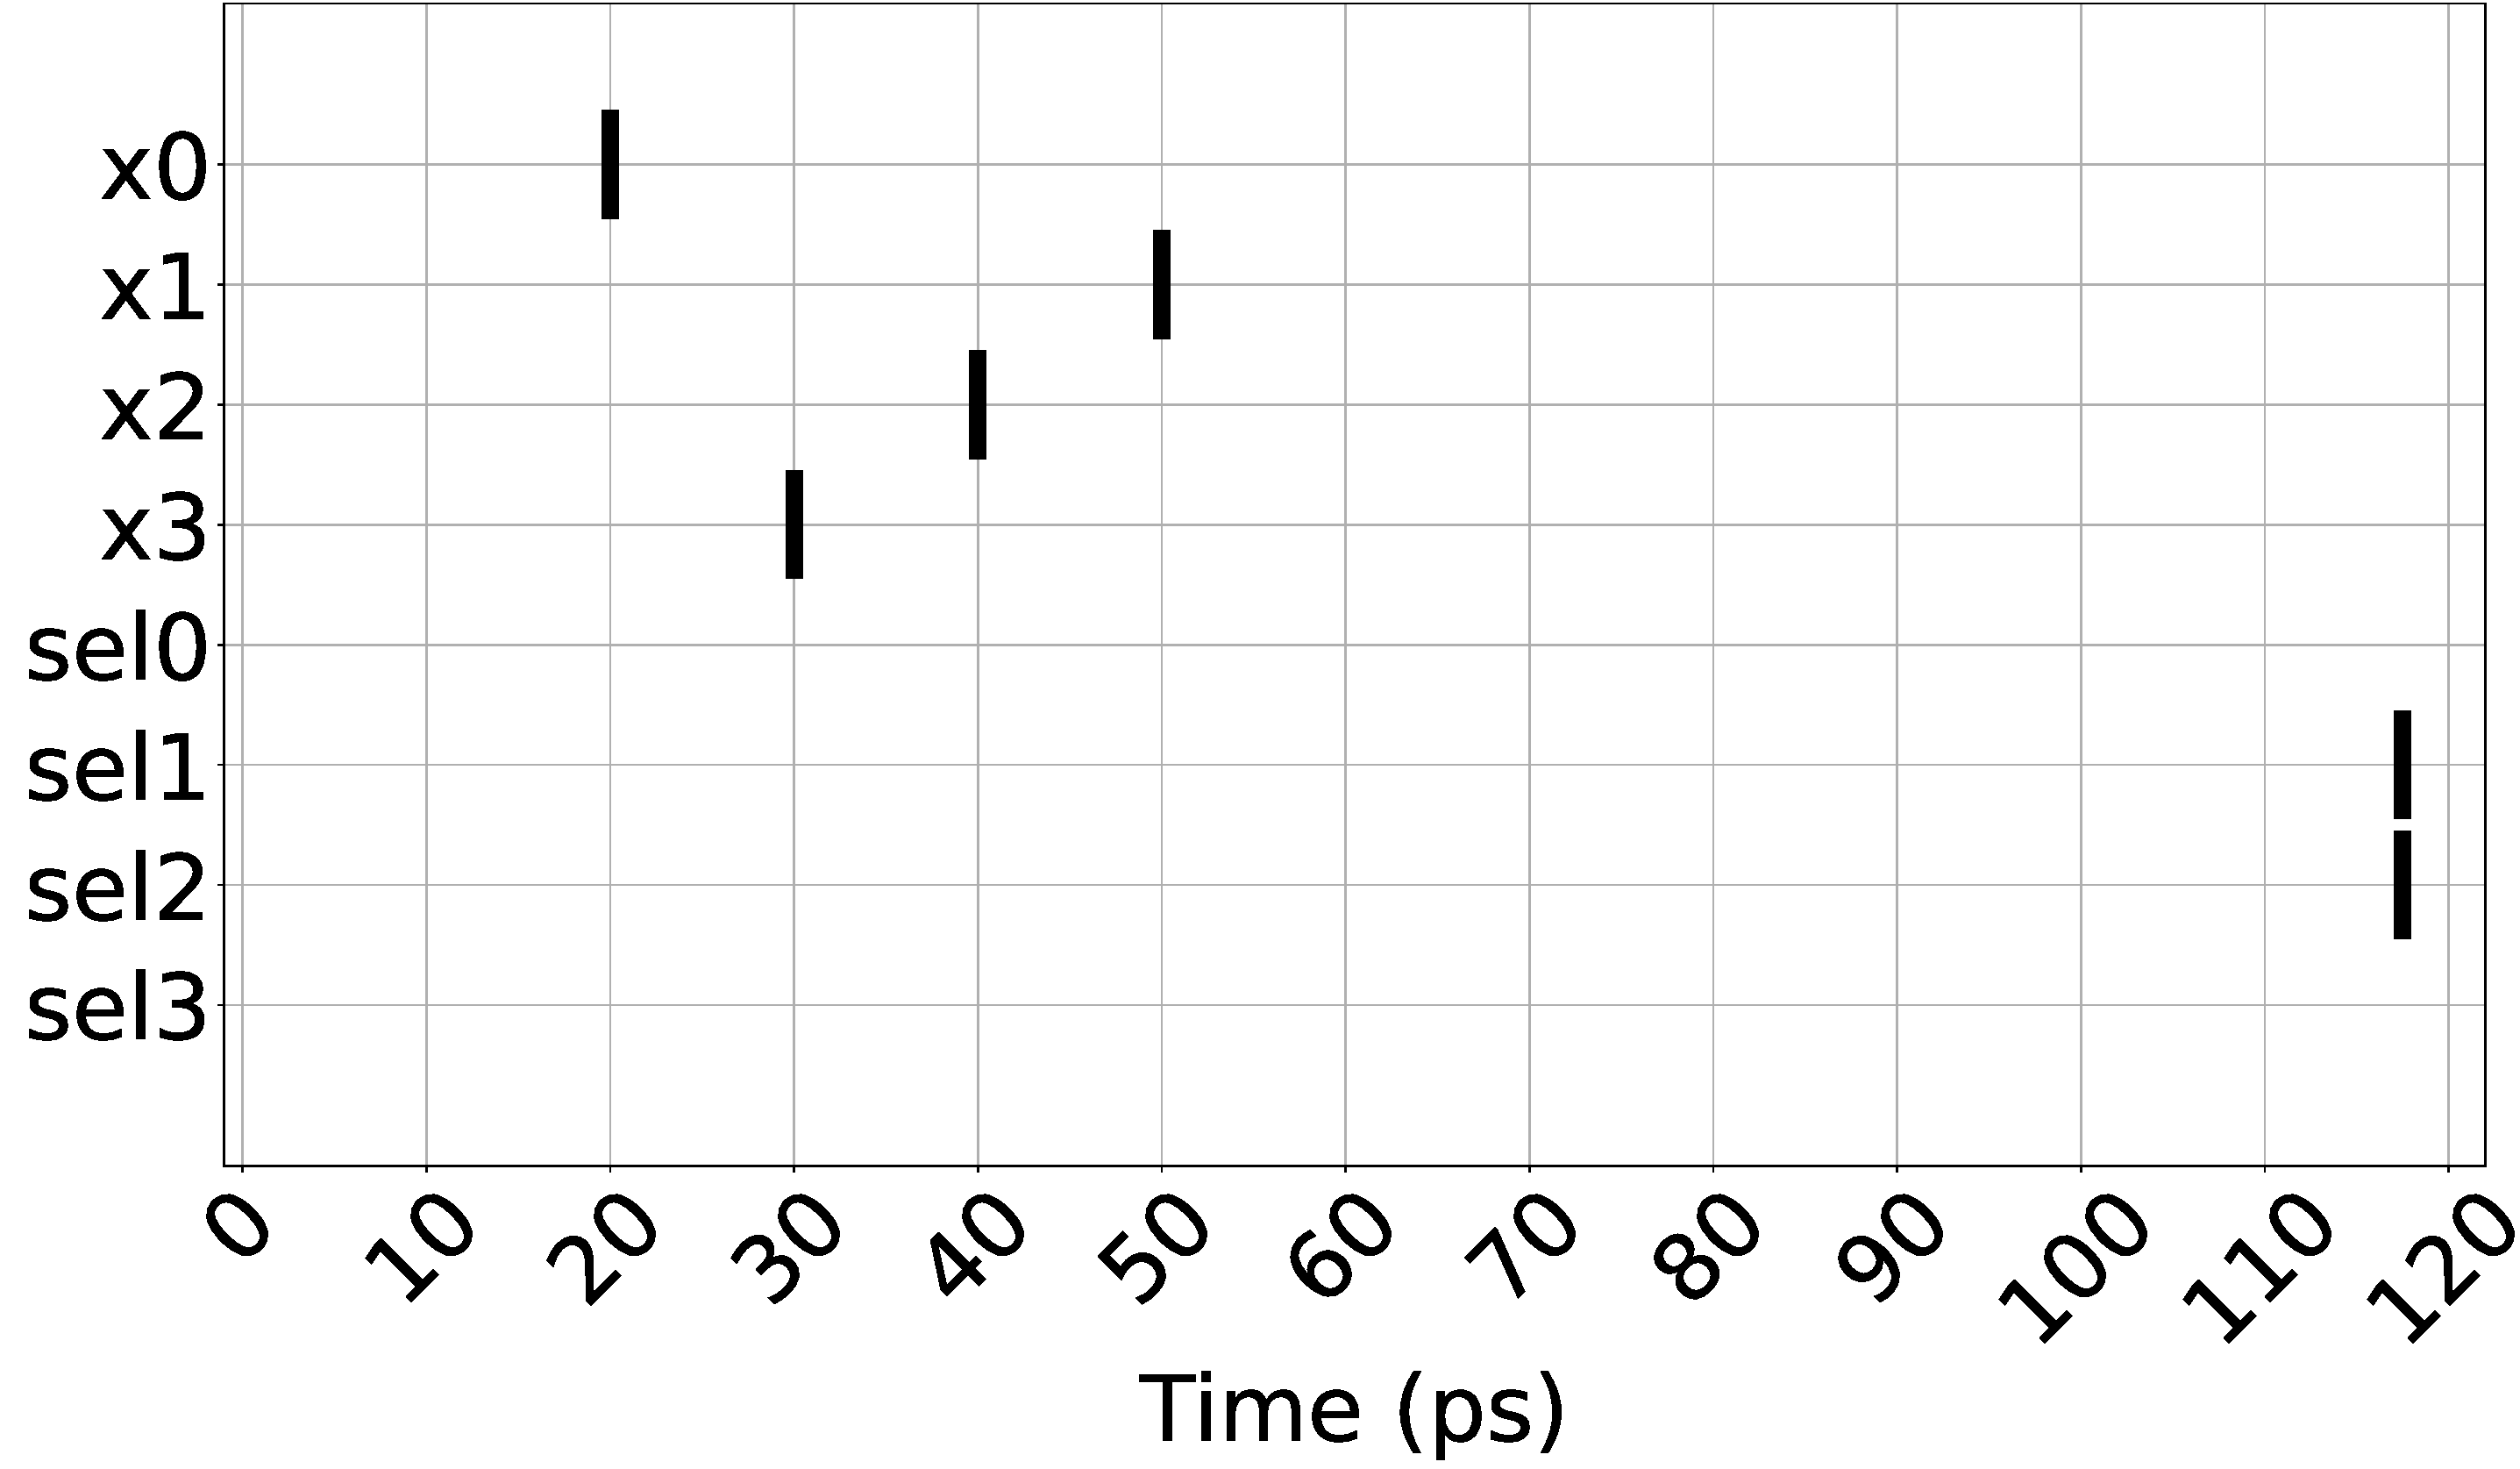
\includegraphics[width=\columnwidth]{figures/simlarge.pdf}
  \end{center}
  \caption{Simulation of arbiter selecting the two highest scoring qubits out of four. The plot shows the time a pulse (indicated by a vertical bar) appears in each of the arbiter's ports. The score of each qubit is encoded in the arrival time of a pulse in the corresponing input port x0 to x3. After a short delay, the arbiter generates pulses at the sel ports of the qubits with the latest arriving inputs. In this case, sel1 and sel2.}\label{fig:pylserun}
\end{figure}


